% Options for packages loaded elsewhere
\PassOptionsToPackage{unicode}{hyperref}
\PassOptionsToPackage{hyphens}{url}
%
\documentclass[
]{article}
\usepackage{amsmath,amssymb}
\usepackage{lmodern}
\usepackage{iftex}
\ifPDFTeX
  \usepackage[T1]{fontenc}
  \usepackage[utf8]{inputenc}
  \usepackage{textcomp} % provide euro and other symbols
\else % if luatex or xetex
  \usepackage{unicode-math}
  \defaultfontfeatures{Scale=MatchLowercase}
  \defaultfontfeatures[\rmfamily]{Ligatures=TeX,Scale=1}
\fi
% Use upquote if available, for straight quotes in verbatim environments
\IfFileExists{upquote.sty}{\usepackage{upquote}}{}
\IfFileExists{microtype.sty}{% use microtype if available
  \usepackage[]{microtype}
  \UseMicrotypeSet[protrusion]{basicmath} % disable protrusion for tt fonts
}{}
\makeatletter
\@ifundefined{KOMAClassName}{% if non-KOMA class
  \IfFileExists{parskip.sty}{%
    \usepackage{parskip}
  }{% else
    \setlength{\parindent}{0pt}
    \setlength{\parskip}{6pt plus 2pt minus 1pt}}
}{% if KOMA class
  \KOMAoptions{parskip=half}}
\makeatother
\usepackage{xcolor}
\usepackage[margin=1in]{geometry}
\usepackage{color}
\usepackage{fancyvrb}
\newcommand{\VerbBar}{|}
\newcommand{\VERB}{\Verb[commandchars=\\\{\}]}
\DefineVerbatimEnvironment{Highlighting}{Verbatim}{commandchars=\\\{\}}
% Add ',fontsize=\small' for more characters per line
\usepackage{framed}
\definecolor{shadecolor}{RGB}{248,248,248}
\newenvironment{Shaded}{\begin{snugshade}}{\end{snugshade}}
\newcommand{\AlertTok}[1]{\textcolor[rgb]{0.94,0.16,0.16}{#1}}
\newcommand{\AnnotationTok}[1]{\textcolor[rgb]{0.56,0.35,0.01}{\textbf{\textit{#1}}}}
\newcommand{\AttributeTok}[1]{\textcolor[rgb]{0.77,0.63,0.00}{#1}}
\newcommand{\BaseNTok}[1]{\textcolor[rgb]{0.00,0.00,0.81}{#1}}
\newcommand{\BuiltInTok}[1]{#1}
\newcommand{\CharTok}[1]{\textcolor[rgb]{0.31,0.60,0.02}{#1}}
\newcommand{\CommentTok}[1]{\textcolor[rgb]{0.56,0.35,0.01}{\textit{#1}}}
\newcommand{\CommentVarTok}[1]{\textcolor[rgb]{0.56,0.35,0.01}{\textbf{\textit{#1}}}}
\newcommand{\ConstantTok}[1]{\textcolor[rgb]{0.00,0.00,0.00}{#1}}
\newcommand{\ControlFlowTok}[1]{\textcolor[rgb]{0.13,0.29,0.53}{\textbf{#1}}}
\newcommand{\DataTypeTok}[1]{\textcolor[rgb]{0.13,0.29,0.53}{#1}}
\newcommand{\DecValTok}[1]{\textcolor[rgb]{0.00,0.00,0.81}{#1}}
\newcommand{\DocumentationTok}[1]{\textcolor[rgb]{0.56,0.35,0.01}{\textbf{\textit{#1}}}}
\newcommand{\ErrorTok}[1]{\textcolor[rgb]{0.64,0.00,0.00}{\textbf{#1}}}
\newcommand{\ExtensionTok}[1]{#1}
\newcommand{\FloatTok}[1]{\textcolor[rgb]{0.00,0.00,0.81}{#1}}
\newcommand{\FunctionTok}[1]{\textcolor[rgb]{0.00,0.00,0.00}{#1}}
\newcommand{\ImportTok}[1]{#1}
\newcommand{\InformationTok}[1]{\textcolor[rgb]{0.56,0.35,0.01}{\textbf{\textit{#1}}}}
\newcommand{\KeywordTok}[1]{\textcolor[rgb]{0.13,0.29,0.53}{\textbf{#1}}}
\newcommand{\NormalTok}[1]{#1}
\newcommand{\OperatorTok}[1]{\textcolor[rgb]{0.81,0.36,0.00}{\textbf{#1}}}
\newcommand{\OtherTok}[1]{\textcolor[rgb]{0.56,0.35,0.01}{#1}}
\newcommand{\PreprocessorTok}[1]{\textcolor[rgb]{0.56,0.35,0.01}{\textit{#1}}}
\newcommand{\RegionMarkerTok}[1]{#1}
\newcommand{\SpecialCharTok}[1]{\textcolor[rgb]{0.00,0.00,0.00}{#1}}
\newcommand{\SpecialStringTok}[1]{\textcolor[rgb]{0.31,0.60,0.02}{#1}}
\newcommand{\StringTok}[1]{\textcolor[rgb]{0.31,0.60,0.02}{#1}}
\newcommand{\VariableTok}[1]{\textcolor[rgb]{0.00,0.00,0.00}{#1}}
\newcommand{\VerbatimStringTok}[1]{\textcolor[rgb]{0.31,0.60,0.02}{#1}}
\newcommand{\WarningTok}[1]{\textcolor[rgb]{0.56,0.35,0.01}{\textbf{\textit{#1}}}}
\usepackage{graphicx}
\makeatletter
\def\maxwidth{\ifdim\Gin@nat@width>\linewidth\linewidth\else\Gin@nat@width\fi}
\def\maxheight{\ifdim\Gin@nat@height>\textheight\textheight\else\Gin@nat@height\fi}
\makeatother
% Scale images if necessary, so that they will not overflow the page
% margins by default, and it is still possible to overwrite the defaults
% using explicit options in \includegraphics[width, height, ...]{}
\setkeys{Gin}{width=\maxwidth,height=\maxheight,keepaspectratio}
% Set default figure placement to htbp
\makeatletter
\def\fps@figure{htbp}
\makeatother
\setlength{\emergencystretch}{3em} % prevent overfull lines
\providecommand{\tightlist}{%
  \setlength{\itemsep}{0pt}\setlength{\parskip}{0pt}}
\setcounter{secnumdepth}{5}
\ifLuaTeX
  \usepackage{selnolig}  % disable illegal ligatures
\fi
\IfFileExists{bookmark.sty}{\usepackage{bookmark}}{\usepackage{hyperref}}
\IfFileExists{xurl.sty}{\usepackage{xurl}}{} % add URL line breaks if available
\urlstyle{same} % disable monospaced font for URLs
\hypersetup{
  pdftitle={p8106\_hw1\_qz2266\_final},
  pdfauthor={Qing Zhou},
  hidelinks,
  pdfcreator={LaTeX via pandoc}}

\title{p8106\_hw1\_qz2266\_final}
\author{Qing Zhou}
\date{}

\begin{document}
\maketitle

{
\setcounter{tocdepth}{2}
\tableofcontents
}
\hypertarget{data-import-and-cleaning}{%
\subsubsection{Data Import and
cleaning}\label{data-import-and-cleaning}}

In this exercise, we predict the sale price of a house using its other
characteristics. The training data are in ``housing train.csv'', and the
test data are in ``housing test.csv''.

\begin{Shaded}
\begin{Highlighting}[]
\CommentTok{\# read in training data}
\NormalTok{train }\OtherTok{=} \FunctionTok{read.csv}\NormalTok{(}\StringTok{"data/housing\_training.csv"}\NormalTok{) }\SpecialCharTok{\%\textgreater{}\%} 
\NormalTok{janitor}\SpecialCharTok{::}\FunctionTok{clean\_names}\NormalTok{()}
\NormalTok{train }\OtherTok{=} \FunctionTok{na.omit}\NormalTok{(train)}

\CommentTok{\# read in test data}
\NormalTok{test }\OtherTok{=} \FunctionTok{read.csv}\NormalTok{(}\StringTok{"data/housing\_test.csv"}\NormalTok{) }\SpecialCharTok{\%\textgreater{}\%} 
\NormalTok{janitor}\SpecialCharTok{::}\FunctionTok{clean\_names}\NormalTok{()}
\NormalTok{test }\OtherTok{=} \FunctionTok{na.omit}\NormalTok{(test)}

\CommentTok{\# create covariates matrix for training and test}
\NormalTok{x\_train }\OtherTok{=} \FunctionTok{model.matrix}\NormalTok{(sale\_price }\SpecialCharTok{\textasciitilde{}}\NormalTok{ ., train)[,}\SpecialCharTok{{-}}\DecValTok{1}\NormalTok{]}
\NormalTok{y\_train }\OtherTok{=}\NormalTok{ train}\SpecialCharTok{$}\NormalTok{sale\_price}
\NormalTok{x\_test }\OtherTok{\textless{}{-}} \FunctionTok{model.matrix}\NormalTok{(sale\_price }\SpecialCharTok{\textasciitilde{}}\NormalTok{ ., test)[ ,}\SpecialCharTok{{-}}\DecValTok{1}\NormalTok{]}
\NormalTok{y\_test }\OtherTok{\textless{}{-}}\NormalTok{ test}\SpecialCharTok{$}\NormalTok{sale\_price}
\end{Highlighting}
\end{Shaded}

Check for potential collinearities among predictors in training data

\begin{Shaded}
\begin{Highlighting}[]
\CommentTok{\# Correlation plot for all predictors}
\FunctionTok{corrplot}\NormalTok{(}\FunctionTok{cor}\NormalTok{(x\_train), }\AttributeTok{method =} \StringTok{"circle"}\NormalTok{, }\AttributeTok{type =} \StringTok{"full"}\NormalTok{, }\AttributeTok{tl.cex =} \FloatTok{0.5}\NormalTok{)}
\end{Highlighting}
\end{Shaded}

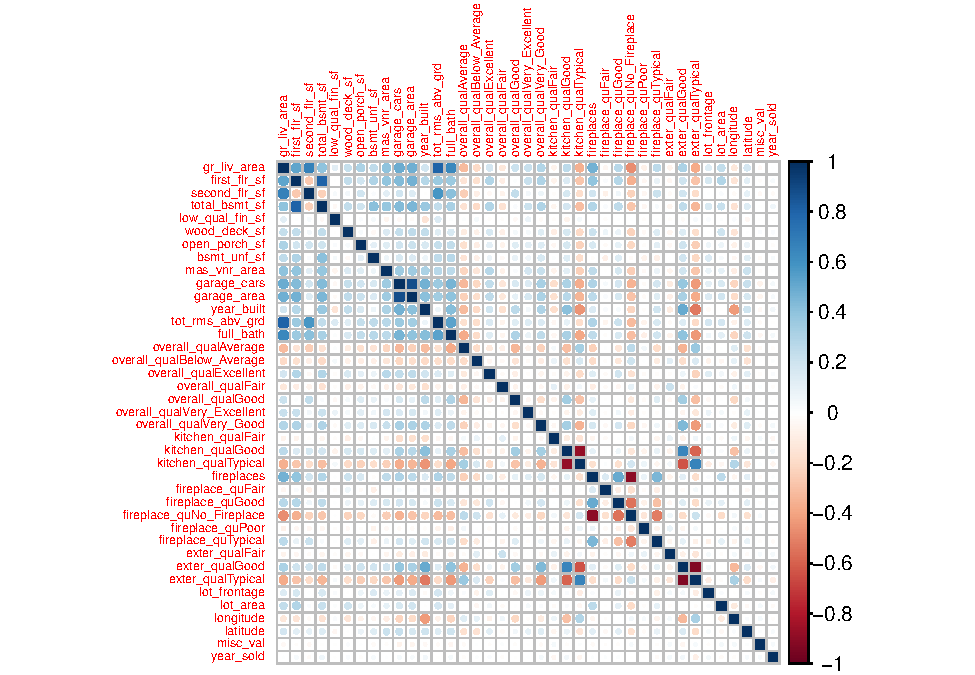
\includegraphics{p8106_hw1_qz2266_final_files/figure-latex/correlation plot-1.pdf}

\begin{itemize}
\item
  From the correlation plot we can see there are high correlations
  between some of the covariates. This high correlation might cause
  collinearity problem.
\item
  To fix the potential multicollinearity issue, regularization methods
  such as lasso, elastic net, or partial least squares could be
  employed, other than linear model. Please see below for these models.
\end{itemize}

\hypertarget{a.-linear-model}{%
\subsubsection{a). Linear model}\label{a.-linear-model}}

\begin{Shaded}
\begin{Highlighting}[]
\FunctionTok{set.seed}\NormalTok{(}\DecValTok{1}\NormalTok{)}
\NormalTok{lm.fit }\OtherTok{\textless{}{-}} \FunctionTok{train}\NormalTok{(x\_train, y\_train, }
             \AttributeTok{method =} \StringTok{"lm"}\NormalTok{,}
             \AttributeTok{trControl =} \FunctionTok{trainControl}\NormalTok{(}\AttributeTok{method =} \StringTok{"repeatedcv"}\NormalTok{, }\AttributeTok{number =} \DecValTok{10}\NormalTok{, }\AttributeTok{repeats =} \DecValTok{5}\NormalTok{))}
\FunctionTok{summary}\NormalTok{(lm.fit)}
\end{Highlighting}
\end{Shaded}

\begin{verbatim}
## 
## Call:
## lm(formula = .outcome ~ ., data = dat)
## 
## Residuals:
##    Min     1Q Median     3Q    Max 
## -89864 -12424    416  12143 140205 
## 
## Coefficients: (1 not defined because of singularities)
##                              Estimate Std. Error t value Pr(>|t|)    
## (Intercept)                -4.985e+06  3.035e+06  -1.642  0.10076    
## gr_liv_area                 2.458e+01  1.393e+01   1.765  0.07778 .  
## first_flr_sf                4.252e+01  1.409e+01   3.017  0.00260 ** 
## second_flr_sf               4.177e+01  1.379e+01   3.029  0.00250 ** 
## total_bsmt_sf               3.519e+01  2.744e+00  12.827  < 2e-16 ***
## low_qual_fin_sf                    NA         NA      NA       NA    
## wood_deck_sf                1.202e+01  4.861e+00   2.474  0.01350 *  
## open_porch_sf               1.618e+01  1.004e+01   1.611  0.10736    
## bsmt_unf_sf                -2.087e+01  1.723e+00 -12.116  < 2e-16 ***
## mas_vnr_area                1.046e+01  4.229e+00   2.473  0.01353 *  
## garage_cars                 4.229e+03  1.893e+03   2.234  0.02563 *  
## garage_area                 7.769e+00  6.497e+00   1.196  0.23195    
## year_built                  3.251e+02  3.130e+01  10.388  < 2e-16 ***
## tot_rms_abv_grd            -3.838e+03  6.922e+02  -5.545 3.51e-08 ***
## full_bath                  -4.341e+03  1.655e+03  -2.622  0.00883 ** 
## overall_qualAverage        -5.013e+03  1.735e+03  -2.890  0.00391 ** 
## overall_qualBelow_Average  -1.280e+04  2.677e+03  -4.782 1.92e-06 ***
## overall_qualExcellent       7.261e+04  5.381e+03  13.494  < 2e-16 ***
## overall_qualFair           -1.115e+04  5.240e+03  -2.127  0.03356 *  
## overall_qualGood            1.226e+04  1.950e+03   6.287 4.30e-10 ***
## overall_qualVery_Excellent  1.304e+05  8.803e+03  14.810  < 2e-16 ***
## overall_qualVery_Good       3.798e+04  2.741e+03  13.852  < 2e-16 ***
## kitchen_qualFair           -2.663e+04  6.325e+03  -4.210 2.71e-05 ***
## kitchen_qualGood           -1.879e+04  4.100e+03  -4.582 5.01e-06 ***
## kitchen_qualTypical        -2.677e+04  4.281e+03  -6.252 5.37e-10 ***
## fireplaces                  1.138e+04  2.257e+03   5.043 5.18e-07 ***
## fireplace_quFair           -7.207e+03  6.823e+03  -1.056  0.29106    
## fireplace_quGood            6.070e+02  5.833e+03   0.104  0.91713    
## fireplace_quNo_Fireplace    3.394e+03  6.298e+03   0.539  0.59002    
## fireplace_quPoor           -5.185e+03  7.399e+03  -0.701  0.48362    
## fireplace_quTypical        -6.398e+03  5.897e+03  -1.085  0.27814    
## exter_qualFair             -3.854e+04  8.383e+03  -4.598 4.66e-06 ***
## exter_qualGood             -1.994e+04  5.585e+03  -3.569  0.00037 ***
## exter_qualTypical          -2.436e+04  5.874e+03  -4.147 3.57e-05 ***
## lot_frontage                1.024e+02  1.905e+01   5.376 8.90e-08 ***
## lot_area                    6.042e-01  7.864e-02   7.683 2.91e-14 ***
## longitude                  -3.481e+04  2.537e+04  -1.372  0.17016    
## latitude                    5.874e+04  3.483e+04   1.686  0.09193 .  
## misc_val                    9.171e-01  1.003e+00   0.914  0.36071    
## year_sold                  -6.455e+02  4.606e+02  -1.401  0.16132    
## ---
## Signif. codes:  0 '***' 0.001 '**' 0.01 '*' 0.05 '.' 0.1 ' ' 1
## 
## Residual standard error: 22190 on 1401 degrees of freedom
## Multiple R-squared:  0.9116, Adjusted R-squared:  0.9092 
## F-statistic: 380.3 on 38 and 1401 DF,  p-value: < 2.2e-16
\end{verbatim}

\begin{Shaded}
\begin{Highlighting}[]
\CommentTok{\# prediction}
\NormalTok{pred.lm }\OtherTok{=} \FunctionTok{predict}\NormalTok{(lm.fit, }\AttributeTok{newdata =}\NormalTok{ x\_test)}
\CommentTok{\# test error}
\NormalTok{lm.rmse }\OtherTok{=} \FunctionTok{RMSE}\NormalTok{(pred.lm, test}\SpecialCharTok{$}\NormalTok{sale\_price); lm.rmse}
\end{Highlighting}
\end{Shaded}

\begin{verbatim}
## [1] 21149.18
\end{verbatim}

\begin{Shaded}
\begin{Highlighting}[]
\NormalTok{lm.mse }\OtherTok{=}\NormalTok{ (lm.rmse}\SpecialCharTok{\^{}}\DecValTok{2}\NormalTok{); lm.mse}
\end{Highlighting}
\end{Shaded}

\begin{verbatim}
## [1] 447287652
\end{verbatim}

Pros and cons of the linear model:

\begin{itemize}
\item
  This model is quite straightforward and easy to fit.The estimates are
  BLUE.The mean-square test error (MSE) for this model is
  \ensuremath{4.4728765\times 10^{8}}.
\item
  However, this model is still quite complicated with too many
  predictors. Moreover, there is multicollinearity issue and potential
  overfitting problem.
\end{itemize}

\hypertarget{b.-lasso-model}{%
\subsubsection{b). Lasso model}\label{b.-lasso-model}}

\hypertarget{lasso-model-1-based-on-lambda-min}{%
\paragraph{lasso model 1 based on lambda
min}\label{lasso-model-1-based-on-lambda-min}}

\begin{Shaded}
\begin{Highlighting}[]
\FunctionTok{set.seed}\NormalTok{(}\DecValTok{1}\NormalTok{)}

\NormalTok{lasso\_fit }\OtherTok{=} \FunctionTok{train}\NormalTok{(x\_train, y\_train, }
                    \AttributeTok{method =} \StringTok{"glmnet"}\NormalTok{,}
                    \AttributeTok{tuneGrid =} \FunctionTok{expand.grid}\NormalTok{(}\AttributeTok{alpha =} \DecValTok{1}\NormalTok{,}
                                           \AttributeTok{lambda =} \FunctionTok{exp}\NormalTok{(}\FunctionTok{seq}\NormalTok{(}\SpecialCharTok{{-}}\DecValTok{2}\NormalTok{, }\DecValTok{8}\NormalTok{, }\AttributeTok{length =} \DecValTok{100}\NormalTok{))),}
                    \AttributeTok{trControl =} \FunctionTok{trainControl}\NormalTok{(}\AttributeTok{method =} \StringTok{"repeatedcv"}\NormalTok{, }\AttributeTok{number =} \DecValTok{10}\NormalTok{, }\AttributeTok{repeats =} \DecValTok{5}\NormalTok{))}

\FunctionTok{plot}\NormalTok{(lasso\_fit, }\AttributeTok{xTrans =}\NormalTok{ log)}
\end{Highlighting}
\end{Shaded}

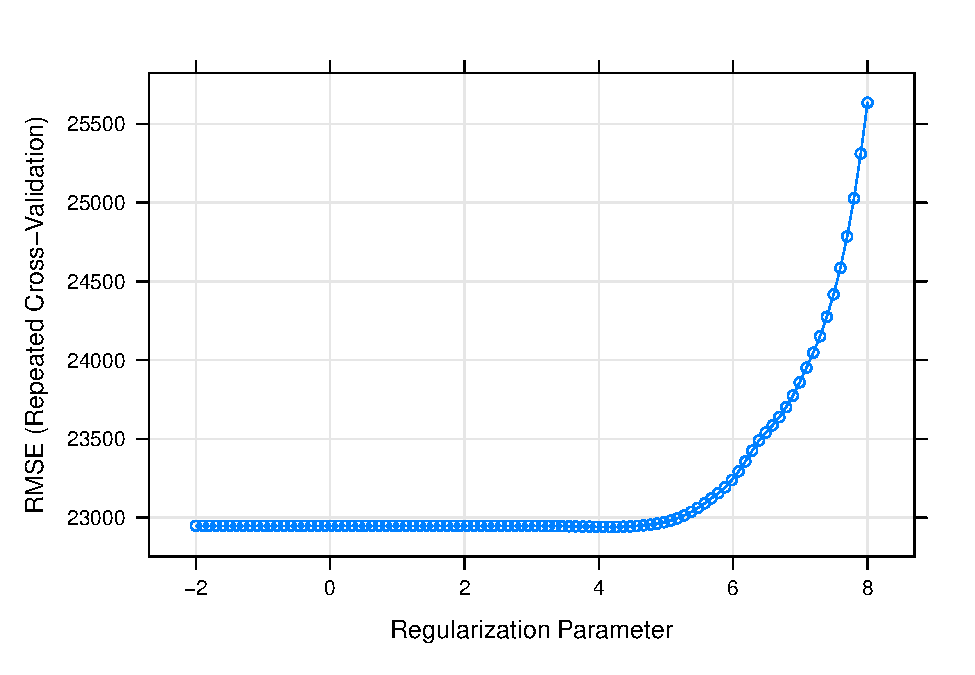
\includegraphics{p8106_hw1_qz2266_final_files/figure-latex/unnamed-chunk-3-1.pdf}

\begin{Shaded}
\begin{Highlighting}[]
\CommentTok{\# optimal tuning parameters}
\NormalTok{lasso\_fit}\SpecialCharTok{$}\NormalTok{bestTune}
\end{Highlighting}
\end{Shaded}

\begin{verbatim}
##    alpha   lambda
## 62     1 64.17516
\end{verbatim}

\begin{Shaded}
\begin{Highlighting}[]
\CommentTok{\# show coefficients}
\FunctionTok{coef}\NormalTok{(lasso\_fit}\SpecialCharTok{$}\NormalTok{finalModel, lasso\_fit}\SpecialCharTok{$}\NormalTok{bestTune}\SpecialCharTok{$}\NormalTok{lambda)}
\end{Highlighting}
\end{Shaded}

\begin{verbatim}
## 40 x 1 sparse Matrix of class "dgCMatrix"
##                                       s1
## (Intercept)                -4.830346e+06
## gr_liv_area                 6.540238e+01
## first_flr_sf                8.016798e-01
## second_flr_sf               .           
## total_bsmt_sf               3.541418e+01
## low_qual_fin_sf            -4.095881e+01
## wood_deck_sf                1.164153e+01
## open_porch_sf               1.544655e+01
## bsmt_unf_sf                -2.088792e+01
## mas_vnr_area                1.089192e+01
## garage_cars                 4.086270e+03
## garage_area                 8.161397e+00
## year_built                  3.233663e+02
## tot_rms_abv_grd            -3.620617e+03
## full_bath                  -3.849455e+03
## overall_qualAverage        -4.856601e+03
## overall_qualBelow_Average  -1.246350e+04
## overall_qualExcellent       7.545290e+04
## overall_qualFair           -1.075910e+04
## overall_qualGood            1.212418e+04
## overall_qualVery_Excellent  1.356218e+05
## overall_qualVery_Good       3.789366e+04
## kitchen_qualFair           -2.487155e+04
## kitchen_qualGood           -1.723010e+04
## kitchen_qualTypical        -2.533814e+04
## fireplaces                  1.055908e+04
## fireplace_quFair           -7.669876e+03
## fireplace_quGood            .           
## fireplace_quNo_Fireplace    1.462970e+03
## fireplace_quPoor           -5.644087e+03
## fireplace_quTypical        -7.011684e+03
## exter_qualFair             -3.340938e+04
## exter_qualGood             -1.515968e+04
## exter_qualTypical          -1.959557e+04
## lot_frontage                9.969303e+01
## lot_area                    6.042705e-01
## longitude                  -3.296544e+04
## latitude                    5.514849e+04
## misc_val                    8.297428e-01
## year_sold                  -5.617527e+02
\end{verbatim}

\begin{Shaded}
\begin{Highlighting}[]
\CommentTok{\# prediction}
\NormalTok{pred\_lasso }\OtherTok{=} \FunctionTok{predict}\NormalTok{(lasso\_fit, }\AttributeTok{newdata =}\NormalTok{ x\_test)}
\CommentTok{\# test error}
\NormalTok{lasso\_mse }\OtherTok{=} \FunctionTok{mean}\NormalTok{((pred\_lasso }\SpecialCharTok{{-}}\NormalTok{ y\_test)}\SpecialCharTok{\^{}}\DecValTok{2}\NormalTok{); lasso\_mse}
\end{Highlighting}
\end{Shaded}

\begin{verbatim}
## [1] 440092572
\end{verbatim}

\begin{Shaded}
\begin{Highlighting}[]
\CommentTok{\# number of predictors}
\NormalTok{num\_coef }\OtherTok{=} \FunctionTok{coef}\NormalTok{(lasso\_fit}\SpecialCharTok{$}\NormalTok{finalModel, lasso\_fit}\SpecialCharTok{$}\NormalTok{bestTune}\SpecialCharTok{$}\NormalTok{lambda) }
\FunctionTok{sum}\NormalTok{(num\_coef }\SpecialCharTok{!=} \DecValTok{0}\NormalTok{) }\SpecialCharTok{{-}} \DecValTok{1}
\end{Highlighting}
\end{Shaded}

\begin{verbatim}
## [1] 37
\end{verbatim}

\hypertarget{lasso-model-2-based-on-1se}{%
\paragraph{lasso model 2 based on
1SE}\label{lasso-model-2-based-on-1se}}

\begin{Shaded}
\begin{Highlighting}[]
\FunctionTok{set.seed}\NormalTok{(}\DecValTok{1}\NormalTok{)}

\NormalTok{lasso\_1se }\OtherTok{=} \FunctionTok{train}\NormalTok{(x\_train, y\_train, }
                  \AttributeTok{method =} \StringTok{"glmnet"}\NormalTok{,}
                  \AttributeTok{tuneGrid =} \FunctionTok{expand.grid}\NormalTok{(}\AttributeTok{alpha =} \DecValTok{1}\NormalTok{,}
                                         \AttributeTok{lambda =} \FunctionTok{exp}\NormalTok{(}\FunctionTok{seq}\NormalTok{(}\SpecialCharTok{{-}}\DecValTok{2}\NormalTok{, }\DecValTok{8}\NormalTok{, }\AttributeTok{length =} \DecValTok{100}\NormalTok{))),}
                  \AttributeTok{trControl =}  \FunctionTok{trainControl}\NormalTok{(}\AttributeTok{method =} \StringTok{"repeatedcv"}\NormalTok{, }\AttributeTok{selectionFunction =} \StringTok{"oneSE"}\NormalTok{, }\AttributeTok{number =} \DecValTok{10}\NormalTok{, }\AttributeTok{repeats =} \DecValTok{5}\NormalTok{))}
                  
\CommentTok{\# optimal tuning parameters based on 1se rule}
\NormalTok{lasso\_1se}\SpecialCharTok{$}\NormalTok{bestTune}
\end{Highlighting}
\end{Shaded}

\begin{verbatim}
##    alpha   lambda
## 80     1 395.3605
\end{verbatim}

\begin{Shaded}
\begin{Highlighting}[]
\CommentTok{\# show coefficients }
\FunctionTok{coef}\NormalTok{(lasso\_1se}\SpecialCharTok{$}\NormalTok{finalModel, lasso\_1se}\SpecialCharTok{$}\NormalTok{bestTune}\SpecialCharTok{$}\NormalTok{lambda)}
\end{Highlighting}
\end{Shaded}

\begin{verbatim}
## 40 x 1 sparse Matrix of class "dgCMatrix"
##                                       s1
## (Intercept)                -3.943441e+06
## gr_liv_area                 6.108086e+01
## first_flr_sf                9.449637e-01
## second_flr_sf               .           
## total_bsmt_sf               3.625951e+01
## low_qual_fin_sf            -3.544140e+01
## wood_deck_sf                1.004751e+01
## open_porch_sf               1.213017e+01
## bsmt_unf_sf                -2.060701e+01
## mas_vnr_area                1.293690e+01
## garage_cars                 3.503770e+03
## garage_area                 9.711868e+00
## year_built                  3.152712e+02
## tot_rms_abv_grd            -2.541684e+03
## full_bath                  -1.469004e+03
## overall_qualAverage        -4.028703e+03
## overall_qualBelow_Average  -1.088208e+04
## overall_qualExcellent       8.701702e+04
## overall_qualFair           -8.812993e+03
## overall_qualGood            1.113742e+04
## overall_qualVery_Excellent  1.557578e+05
## overall_qualVery_Good       3.731931e+04
## kitchen_qualFair           -1.452506e+04
## kitchen_qualGood           -7.943206e+03
## kitchen_qualTypical        -1.672289e+04
## fireplaces                  8.251261e+03
## fireplace_quFair           -3.942182e+03
## fireplace_quGood            2.111321e+03
## fireplace_quNo_Fireplace    .           
## fireplace_quPoor           -1.621801e+03
## fireplace_quTypical        -4.236539e+03
## exter_qualFair             -1.699637e+04
## exter_qualGood              .           
## exter_qualTypical          -4.789838e+03
## lot_frontage                8.694872e+01
## lot_area                    5.920132e-01
## longitude                  -2.270960e+04
## latitude                    3.807773e+04
## misc_val                    3.236657e-01
## year_sold                  -1.732609e+02
\end{verbatim}

\begin{Shaded}
\begin{Highlighting}[]
\CommentTok{\# prediction}
\NormalTok{pred\_lasso\_1se }\OtherTok{=} \FunctionTok{predict}\NormalTok{(lasso\_1se, }\AttributeTok{newdata =}\NormalTok{ x\_test)}
\CommentTok{\# test error}
\NormalTok{lasso\_1se\_mse }\OtherTok{=} \FunctionTok{mean}\NormalTok{((pred\_lasso\_1se }\SpecialCharTok{{-}}\NormalTok{ y\_test)}\SpecialCharTok{\^{}}\DecValTok{2}\NormalTok{); lasso\_1se\_mse}
\end{Highlighting}
\end{Shaded}

\begin{verbatim}
## [1] 420909622
\end{verbatim}

\begin{Shaded}
\begin{Highlighting}[]
\CommentTok{\# number of predictors}
\NormalTok{num\_coef\_1se }\OtherTok{=} \FunctionTok{coef}\NormalTok{(lasso\_1se}\SpecialCharTok{$}\NormalTok{finalModel, lasso\_1se}\SpecialCharTok{$}\NormalTok{bestTune}\SpecialCharTok{$}\NormalTok{lambda) }
\FunctionTok{sum}\NormalTok{(num\_coef\_1se }\SpecialCharTok{!=} \DecValTok{0}\NormalTok{) }\SpecialCharTok{{-}} \DecValTok{1}
\end{Highlighting}
\end{Shaded}

\begin{verbatim}
## [1] 36
\end{verbatim}

\begin{itemize}
\item
  There are 37 predictors in lasso model 1 based on lambda min, and 36
  predictors in lasso model 2 based on 1se rule.
\item
  The selected turing parameters for lowest cv rmse are alpha=1 and
  lambda=64.18 in lasso model 1. When the 1se rule is applied to lasso
  model 2, lambda changes to 395.36.
\item
  Lasso model 2 based on 1se rule has smaller test MSE which is
  \ensuremath{4.2090962\times 10^{8}} than lasso model 1 based on lambda
  min which is \ensuremath{4.4009257\times 10^{8}}. Therefore, lasso
  model 2 based on 1se is better.
\end{itemize}

\hypertarget{c.-elastic-net-model}{%
\subsubsection{c). Elastic Net model}\label{c.-elastic-net-model}}

\hypertarget{elastice-net-model-1}{%
\paragraph{Elastice net model 1}\label{elastice-net-model-1}}

\begin{Shaded}
\begin{Highlighting}[]
\FunctionTok{set.seed}\NormalTok{(}\DecValTok{1}\NormalTok{)}

\NormalTok{elnet\_fit }\OtherTok{=} \FunctionTok{train}\NormalTok{(x\_train, y\_train, }
                  \AttributeTok{method =} \StringTok{"glmnet"}\NormalTok{,}
                  \AttributeTok{tuneGrid =} \FunctionTok{expand.grid}\NormalTok{(}\AttributeTok{alpha =} \FunctionTok{seq}\NormalTok{(}\DecValTok{0}\NormalTok{, }\DecValTok{1}\NormalTok{, }\AttributeTok{length =} \DecValTok{21}\NormalTok{),}
                                         \AttributeTok{lambda =} \FunctionTok{exp}\NormalTok{(}\FunctionTok{seq}\NormalTok{(}\SpecialCharTok{{-}}\DecValTok{2}\NormalTok{, }\DecValTok{8}\NormalTok{, }\AttributeTok{length =} \DecValTok{50}\NormalTok{))),}
                  \AttributeTok{trControl =} \FunctionTok{trainControl}\NormalTok{(}\AttributeTok{method =} \StringTok{"repeatedcv"}\NormalTok{, }\AttributeTok{number =} \DecValTok{10}\NormalTok{, }\AttributeTok{repeats =} \DecValTok{5}\NormalTok{))}

\CommentTok{\# visualization}
\NormalTok{myCol }\OtherTok{\textless{}{-}} \FunctionTok{rainbow}\NormalTok{(}\DecValTok{25}\NormalTok{)}
\NormalTok{myPar }\OtherTok{\textless{}{-}} \FunctionTok{list}\NormalTok{(}\AttributeTok{superpose.symbol =} \FunctionTok{list}\NormalTok{(}\AttributeTok{col =}\NormalTok{ myCol),}
\AttributeTok{superpose.line =} \FunctionTok{list}\NormalTok{(}\AttributeTok{col =}\NormalTok{ myCol))}
\FunctionTok{plot}\NormalTok{(elnet\_fit, }\AttributeTok{par.settings =}\NormalTok{ myPar)}
\end{Highlighting}
\end{Shaded}

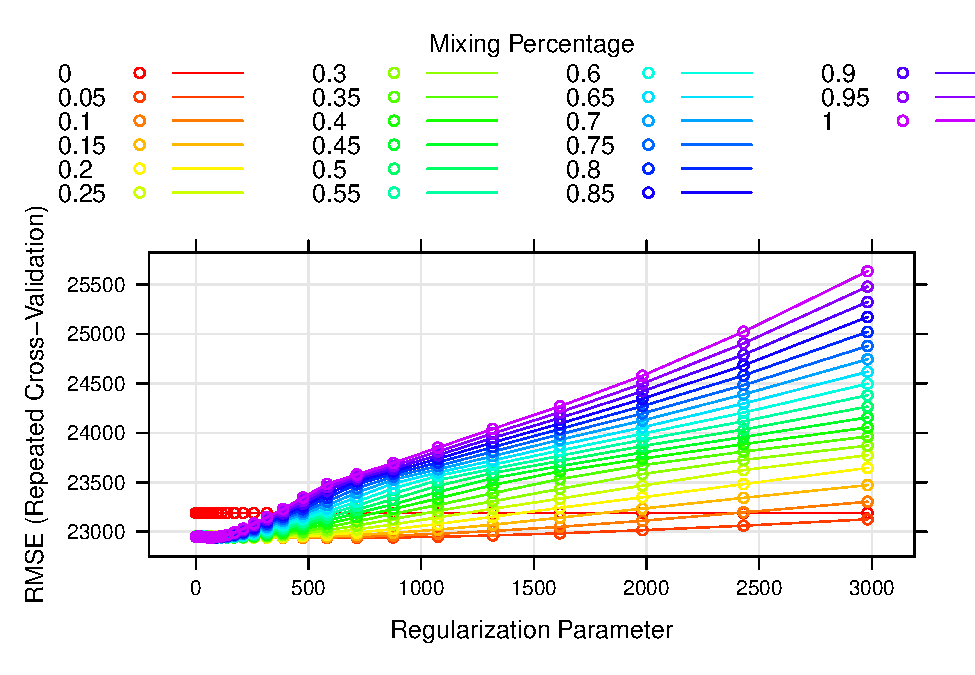
\includegraphics{p8106_hw1_qz2266_final_files/figure-latex/unnamed-chunk-6-1.pdf}

\begin{Shaded}
\begin{Highlighting}[]
\CommentTok{\# tuning parameter }
\NormalTok{elnet\_fit}\SpecialCharTok{$}\NormalTok{bestTune}
\end{Highlighting}
\end{Shaded}

\begin{verbatim}
##    alpha   lambda
## 92  0.05 582.5103
\end{verbatim}

\begin{Shaded}
\begin{Highlighting}[]
\CommentTok{\# show coefficients}
\FunctionTok{coef}\NormalTok{(elnet\_fit}\SpecialCharTok{$}\NormalTok{finalModel, elnet\_fit}\SpecialCharTok{$}\NormalTok{bestTune}\SpecialCharTok{$}\NormalTok{lambda)}
\end{Highlighting}
\end{Shaded}

\begin{verbatim}
## 40 x 1 sparse Matrix of class "dgCMatrix"
##                                       s1
## (Intercept)                -5.112549e+06
## gr_liv_area                 3.877324e+01
## first_flr_sf                2.669846e+01
## second_flr_sf               2.545218e+01
## total_bsmt_sf               3.494244e+01
## low_qual_fin_sf            -1.586458e+01
## wood_deck_sf                1.232562e+01
## open_porch_sf               1.688120e+01
## bsmt_unf_sf                -2.072755e+01
## mas_vnr_area                1.165596e+01
## garage_cars                 4.046453e+03
## garage_area                 8.893308e+00
## year_built                  3.191927e+02
## tot_rms_abv_grd            -3.440136e+03
## full_bath                  -3.692753e+03
## overall_qualAverage        -5.116812e+03
## overall_qualBelow_Average  -1.270813e+04
## overall_qualExcellent       7.582763e+04
## overall_qualFair           -1.147347e+04
## overall_qualGood            1.198272e+04
## overall_qualVery_Excellent  1.363894e+05
## overall_qualVery_Good       3.765814e+04
## kitchen_qualFair           -2.368649e+04
## kitchen_qualGood           -1.610599e+04
## kitchen_qualTypical        -2.415667e+04
## fireplaces                  1.082895e+04
## fireplace_quFair           -7.857833e+03
## fireplace_quGood            1.486635e+02
## fireplace_quNo_Fireplace    1.819327e+03
## fireplace_quPoor           -5.804038e+03
## fireplace_quTypical        -6.962451e+03
## exter_qualFair             -3.296303e+04
## exter_qualGood             -1.455999e+04
## exter_qualTypical          -1.915475e+04
## lot_frontage                1.001690e+02
## lot_area                    6.032320e-01
## longitude                  -3.515266e+04
## latitude                    5.775817e+04
## misc_val                    8.684001e-01
## year_sold                  -5.747735e+02
\end{verbatim}

\begin{Shaded}
\begin{Highlighting}[]
\CommentTok{\# prediction}
\NormalTok{pred\_elnet }\OtherTok{=} \FunctionTok{predict}\NormalTok{(elnet\_fit, }\AttributeTok{newdata =}\NormalTok{ x\_test)}
\CommentTok{\# test error}
\NormalTok{elnet\_mse }\OtherTok{=} \FunctionTok{mean}\NormalTok{(}\FunctionTok{RMSE}\NormalTok{(pred\_elnet, y\_test)}\SpecialCharTok{\^{}}\DecValTok{2}\NormalTok{); elnet\_mse}
\end{Highlighting}
\end{Shaded}

\begin{verbatim}
## [1] 438591167
\end{verbatim}

\hypertarget{elastic-net-model-2-based-on-1se}{%
\paragraph{Elastic net model 2 based on
1se}\label{elastic-net-model-2-based-on-1se}}

\begin{Shaded}
\begin{Highlighting}[]
\FunctionTok{set.seed}\NormalTok{(}\DecValTok{1}\NormalTok{)}
\CommentTok{\# try to fit elastic net model applying 1se rule to select tuning parameters}
\NormalTok{elnet\_1se }\OtherTok{=} \FunctionTok{train}\NormalTok{(x\_train, y\_train, }
                    \AttributeTok{method =} \StringTok{"glmnet"}\NormalTok{,}
                    \AttributeTok{tuneGrid =} \FunctionTok{expand.grid}\NormalTok{(}\AttributeTok{alpha =} \FunctionTok{seq}\NormalTok{(}\DecValTok{0}\NormalTok{, }\DecValTok{1}\NormalTok{, }\AttributeTok{length =} \DecValTok{21}\NormalTok{),}
                                           \AttributeTok{lambda =} \FunctionTok{exp}\NormalTok{(}\FunctionTok{seq}\NormalTok{(}\SpecialCharTok{{-}}\DecValTok{2}\NormalTok{, }\DecValTok{8}\NormalTok{, }\AttributeTok{length =} \DecValTok{50}\NormalTok{))),}
                    \AttributeTok{trControl =}  \FunctionTok{trainControl}\NormalTok{(}\AttributeTok{method =} \StringTok{"repeatedcv"}\NormalTok{, }\AttributeTok{selectionFunction =} \StringTok{"oneSE"}\NormalTok{, }\AttributeTok{number =} \DecValTok{10}\NormalTok{, }\AttributeTok{repeats =} \DecValTok{5}\NormalTok{))}

\CommentTok{\# tuning parameters}
\NormalTok{elnet\_1se}\SpecialCharTok{$}\NormalTok{bestTune}
\end{Highlighting}
\end{Shaded}

\begin{verbatim}
##    alpha   lambda
## 50     0 2980.958
\end{verbatim}

\begin{Shaded}
\begin{Highlighting}[]
\CommentTok{\# show coefficients }
\FunctionTok{coef}\NormalTok{(elnet\_1se}\SpecialCharTok{$}\NormalTok{finalModel, elnet\_1se}\SpecialCharTok{$}\NormalTok{bestTune}\SpecialCharTok{$}\NormalTok{lambda)}
\end{Highlighting}
\end{Shaded}

\begin{verbatim}
## 40 x 1 sparse Matrix of class "dgCMatrix"
##                                       s1
## (Intercept)                -6.335390e+06
## gr_liv_area                 3.239590e+01
## first_flr_sf                2.625217e+01
## second_flr_sf               2.206668e+01
## total_bsmt_sf               3.197020e+01
## low_qual_fin_sf            -1.786580e+01
## wood_deck_sf                1.581469e+01
## open_porch_sf               2.360529e+01
## bsmt_unf_sf                -1.879961e+01
## mas_vnr_area                1.765883e+01
## garage_cars                 3.835315e+03
## garage_area                 1.380900e+01
## year_built                  2.840685e+02
## tot_rms_abv_grd            -1.777713e+03
## full_bath                  -1.514764e+03
## overall_qualAverage        -5.989414e+03
## overall_qualBelow_Average  -1.282769e+04
## overall_qualExcellent       7.581098e+04
## overall_qualFair           -1.422795e+04
## overall_qualGood            9.779199e+03
## overall_qualVery_Excellent  1.397774e+05
## overall_qualVery_Good       3.386129e+04
## kitchen_qualFair           -1.663421e+04
## kitchen_qualGood           -9.438848e+03
## kitchen_qualTypical        -1.770321e+04
## fireplaces                  9.919400e+03
## fireplace_quFair           -7.656381e+03
## fireplace_quGood            1.644805e+03
## fireplace_quNo_Fireplace    3.759105e+02
## fireplace_quPoor           -5.682051e+03
## fireplace_quTypical        -5.611492e+03
## exter_qualFair             -2.585950e+04
## exter_qualGood             -6.657289e+03
## exter_qualTypical          -1.321177e+04
## lot_frontage                9.486833e+01
## lot_area                    5.855032e-01
## longitude                  -4.434608e+04
## latitude                    6.263526e+04
## misc_val                    8.342702e-01
## year_sold                  -4.693104e+02
\end{verbatim}

\begin{Shaded}
\begin{Highlighting}[]
\CommentTok{\# prediction}
\NormalTok{pred\_elnet\_1se }\OtherTok{=} \FunctionTok{predict}\NormalTok{(elnet\_1se, }\AttributeTok{newdata =}\NormalTok{ x\_test)}
\CommentTok{\# test error}
\NormalTok{elnet\_mse\_1se }\OtherTok{=} \FunctionTok{mean}\NormalTok{(}\FunctionTok{RMSE}\NormalTok{(pred\_elnet\_1se, y\_test)}\SpecialCharTok{\^{}}\DecValTok{2}\NormalTok{); elnet\_mse\_1se}
\end{Highlighting}
\end{Shaded}

\begin{verbatim}
## [1] 426357707
\end{verbatim}

\begin{itemize}
\item
  The selected tuning parameters of elastic net model 1 is alpha = 0.05
  and lambda = 582.5 and test error is
  \ensuremath{4.3859117\times 10^{8}}. If 1se rule is applied to elastic
  net model, the tuning parameters is alpha = 0 and lambda is 2980.96,
  and test error is \ensuremath{4.2635771\times 10^{8}} .
\item
  As we know, elastic net allows us to tune the alpha parameter where
  alpha = 0 corresponds to ridge and alpha = 1 to lasso. That means we
  can choose an alpha value between 0 and 1 to optimize the elastic net.
  In elastic net model 2, we found alpha = 0. Therefore, the penalty
  function reduces to the ridge term. Thus, we don't need to apply 1se
  rule to select tuning parameters in this elastic net model. It doesn't
  help to optimize this model.
\end{itemize}

\hypertarget{d.-partial-least-squares-model}{%
\subsubsection{d). Partial least squares
model}\label{d.-partial-least-squares-model}}

\begin{Shaded}
\begin{Highlighting}[]
\FunctionTok{set.seed}\NormalTok{(}\DecValTok{1}\NormalTok{)}

\NormalTok{pls\_fit }\OtherTok{\textless{}{-}} \FunctionTok{train}\NormalTok{(x\_train, y\_train,}
                 \AttributeTok{method =} \StringTok{"pls"}\NormalTok{,}
                 \AttributeTok{tuneGrid =} \FunctionTok{data.frame}\NormalTok{(}\AttributeTok{ncomp =} \DecValTok{1}\SpecialCharTok{:}\DecValTok{19}\NormalTok{),}
                 \AttributeTok{trControl =}  \FunctionTok{trainControl}\NormalTok{(}\AttributeTok{method =} \StringTok{"repeatedcv"}\NormalTok{, }\AttributeTok{number =} \DecValTok{10}\NormalTok{, }\AttributeTok{repeats =} \DecValTok{5}\NormalTok{),}
                 \AttributeTok{preProcess =} \FunctionTok{c}\NormalTok{(}\StringTok{"center"}\NormalTok{, }\StringTok{"scale"}\NormalTok{))}
\FunctionTok{summary}\NormalTok{(pls\_fit)}
\end{Highlighting}
\end{Shaded}

\begin{verbatim}
## Data:    X dimension: 1440 39 
##  Y dimension: 1440 1
## Fit method: oscorespls
## Number of components considered: 12
## TRAINING: % variance explained
##           1 comps  2 comps  3 comps  4 comps  5 comps  6 comps  7 comps
## X           20.02    25.93    29.67    33.59    37.01    40.03    42.49
## .outcome    79.73    86.35    89.36    90.37    90.87    90.99    91.06
##           8 comps  9 comps  10 comps  11 comps  12 comps
## X           45.53    47.97     50.15     52.01     53.69
## .outcome    91.08    91.10     91.13     91.15     91.15
\end{verbatim}

\begin{Shaded}
\begin{Highlighting}[]
\FunctionTok{ggplot}\NormalTok{(pls\_fit, }\AttributeTok{highlight =} \ConstantTok{TRUE}\NormalTok{) }\SpecialCharTok{+}  
\FunctionTok{scale\_x\_continuous}\NormalTok{(}\AttributeTok{breaks =} \FunctionTok{seq}\NormalTok{(}\DecValTok{0}\NormalTok{,}\DecValTok{20}\NormalTok{,}\AttributeTok{by =} \DecValTok{1}\NormalTok{))}
\end{Highlighting}
\end{Shaded}

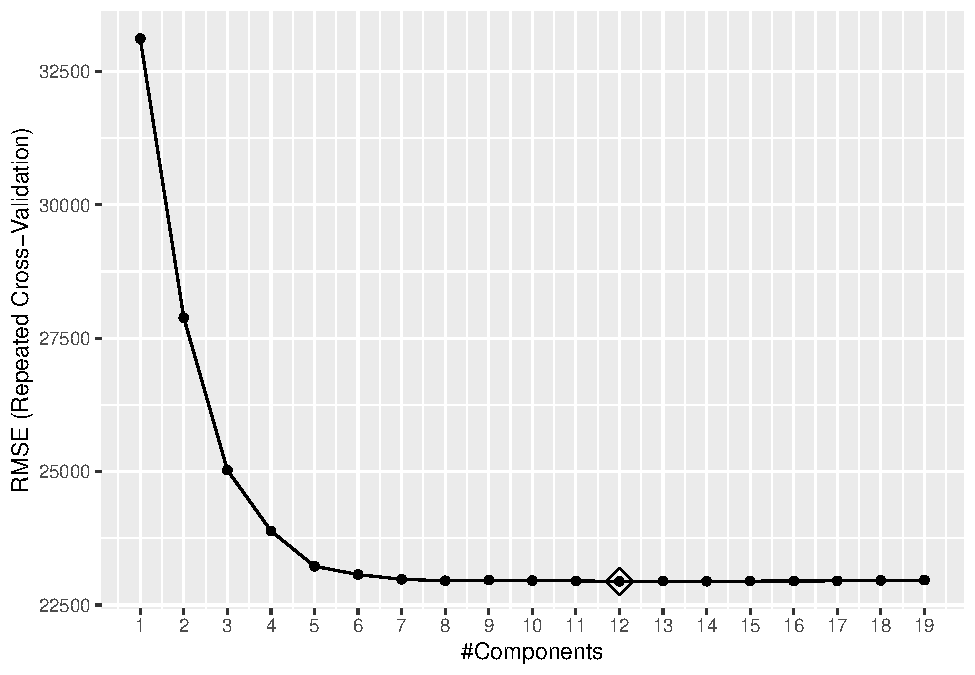
\includegraphics{p8106_hw1_qz2266_final_files/figure-latex/unnamed-chunk-9-1.pdf}

\begin{Shaded}
\begin{Highlighting}[]
\CommentTok{\# prediction}
\NormalTok{pls\_pred }\OtherTok{=} \FunctionTok{predict}\NormalTok{(pls\_fit, }\AttributeTok{newdata =}\NormalTok{ x\_test)}
\CommentTok{\# test error}
\NormalTok{pls\_mse }\OtherTok{=} \FunctionTok{mean}\NormalTok{((pls\_pred }\SpecialCharTok{{-}}\NormalTok{ y\_test)}\SpecialCharTok{\^{}}\DecValTok{2}\NormalTok{); pls\_mse}
\end{Highlighting}
\end{Shaded}

\begin{verbatim}
## [1] 449622718
\end{verbatim}

From the summary of this partial least squares model we found the number
of components is 12. The test error is
\ensuremath{4.4962272\times 10^{8}}.

\hypertarget{model-comparison}{%
\paragraph{Model comparison}\label{model-comparison}}

\begin{Shaded}
\begin{Highlighting}[]
\FunctionTok{set.seed}\NormalTok{(}\DecValTok{1}\NormalTok{)}

\CommentTok{\# compare four models}
\NormalTok{resamp }\OtherTok{\textless{}{-}} \FunctionTok{resamples}\NormalTok{(}\FunctionTok{list}\NormalTok{(}\AttributeTok{least\_square =}\NormalTok{ lm.fit, }\AttributeTok{lasso =}\NormalTok{ lasso\_1se, }\AttributeTok{elastic\_net =}\NormalTok{ elnet\_fit, }\AttributeTok{pls =}\NormalTok{ pls\_fit))}
\FunctionTok{summary}\NormalTok{(resamp)}
\end{Highlighting}
\end{Shaded}

\begin{verbatim}
## 
## Call:
## summary.resamples(object = resamp)
## 
## Models: least_square, lasso, elastic_net, pls 
## Number of resamples: 50 
## 
## MAE 
##                  Min.  1st Qu.   Median     Mean  3rd Qu.     Max. NA's
## least_square 13590.23 16046.61 16694.90 16712.84 17491.07 19148.35    0
## lasso        13612.12 16032.47 16832.86 16653.34 17423.12 19210.70    0
## elastic_net  13491.87 15930.93 16567.62 16626.55 17392.02 19166.44    0
## pls          13541.68 16090.73 16727.26 16716.20 17492.65 19113.09    0
## 
## RMSE 
##                  Min.  1st Qu.   Median     Mean  3rd Qu.     Max. NA's
## least_square 17991.36 21596.77 22880.98 22978.67 24085.83 29899.57    0
## lasso        18249.56 21725.37 23428.71 23238.78 24452.90 30382.60    0
## elastic_net  17875.42 21562.96 23017.69 22936.08 24166.08 29953.16    0
## pls          17907.12 21463.52 23008.08 22943.72 24070.28 29535.42    0
## 
## Rsquared 
##                   Min.   1st Qu.    Median      Mean   3rd Qu.      Max. NA's
## least_square 0.8600209 0.8924164 0.9059332 0.9028661 0.9149852 0.9387696    0
## lasso        0.8593599 0.8916075 0.9038168 0.9009386 0.9118428 0.9364788    0
## elastic_net  0.8603607 0.8931148 0.9069545 0.9032441 0.9146375 0.9393932    0
## pls          0.8603467 0.8921784 0.9071393 0.9030770 0.9155912 0.9392286    0
\end{verbatim}

\begin{Shaded}
\begin{Highlighting}[]
\CommentTok{\# make a boxplot to show RMSE of 4 models}
\FunctionTok{bwplot}\NormalTok{(resamp, }\AttributeTok{metric =} \StringTok{"RMSE"}\NormalTok{)}
\end{Highlighting}
\end{Shaded}

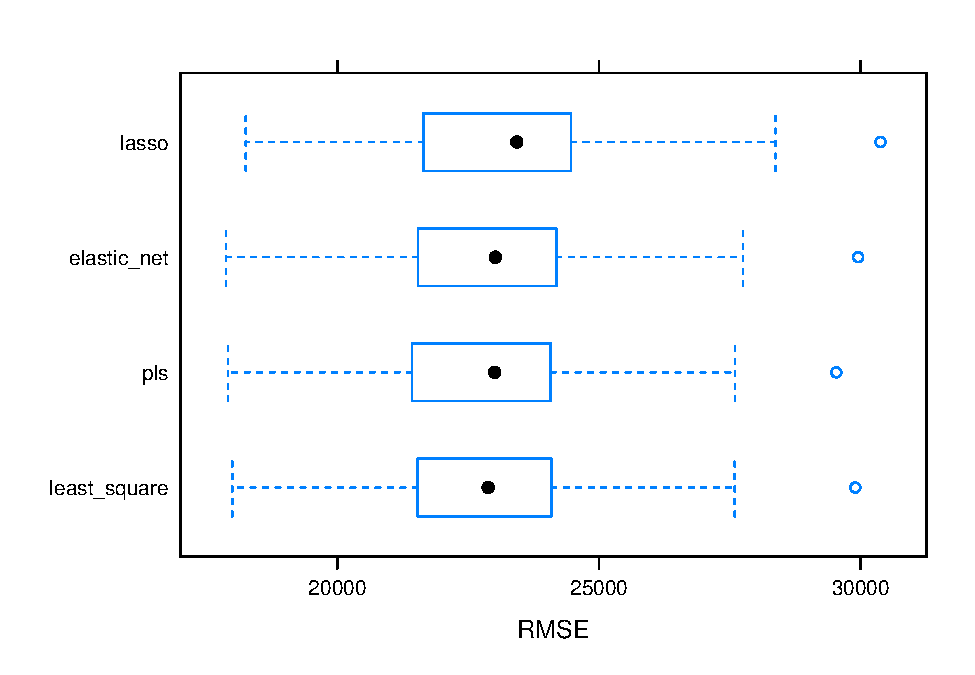
\includegraphics{p8106_hw1_qz2266_final_files/figure-latex/boxplot-1.pdf}

\begin{itemize}
\item
  As we discussed above, linear model has multiple downsides such as
  violation of the principle of parsimony, multicollinearity, etc.
\item
  As for the rest 3 models, from the summary and boxplot we found
  elastic net model has the lowest RMSE, lowest MAE, as well as highest
  R\_squred. In addition, it's more difficult to interpret the results
  of partial least squares model.
\item
  Therefore, I will choose elastic net model as the final model for
  predicting the response.
\end{itemize}

\end{document}
